\documentclass[liststotoc,bibtotoc,fontsize=14pt,]{scrreprt}
\usepackage[utf8]{inputenc} % Zeichenkodierung
\usepackage[ngerman]{babel} % neue deutsche Rechtschreibung
\usepackage{etoolbox}
\setlength{\footskip}{30pt}
\apptocmd{\thebibliography}{\raggedright}{}{}
\usepackage{graphicx}
\usepackage{caption}
\usepackage{subcaption}
\usepackage{url}
\usepackage[onehalfspacing]{setspace}
\usepackage{breakurl}
\usepackage{float}
\usepackage[table,xcdraw]{xcolor}
\usepackage{tabularx}
\usepackage[breaklinks]{hyperref}
\def\UrlBreaks{\do\/\do-}
\usepackage{tocloft}
\usepackage{chngcntr}
\usepackage{listings}
\usepackage{color}
\usepackage[parfill]{parskip}
\definecolor{lightgray}{rgb}{.9,.9,.9}
\definecolor{darkgray}{rgb}{.4,.4,.4} 
\definecolor{purple}{rgb}{0.65, 0.12, 0.82}

\counterwithout{footnote}{chapter}

\deffootnote[2em]{2em}{2em}{%
	\makebox[2em][l]{\bfseries\thefootnotemark}}

\renewcommand{\cftchapdotsep}{\cftdotsep}
\renewcommand{\cftchapleader}{\cftdotfill{\cftchapdotsep}}
\usepackage{amsmath}
\usepackage[paper=a4paper,left=30mm,right=30mm,top=25mm,bottom=25mm]{geometry}
\usepackage[section]{placeins}
\usepackage[font=small,justification=justified]{caption}
\newcommand{\namesigdate}[3][Ort, Datum]{%
	\parbox{\textwidth}{
		\raggedleft #3 
		\vspace{2cm}
		
		\parbox{5cm}{
			\raggedright
			\rule{6cm}{1pt}\\
			#1 
		}
		\hfill
		\parbox{5cm}{
			\raggedright
			\rule{6cm}{1pt}\\
			#2
		}
	}
}


\newcommand*{\tabularwidth}{}
\newdimen\tabularwidth
\usepackage{minitoc}
\hypersetup{
	colorlinks,
	citecolor=black,
	filecolor=black,
	linkcolor=black,
	urlcolor=black
}


\title{Dokumentation Stereo-Fotografie}
\author{Sebastian Degner}

\begin{document}
	%\maketitle
	
	\begin{titlepage}
		\begin{center}
			\vspace{2cm}
			Dokumentation\\ \textbf{Multishot-Technik in der digitalen Fotografie}\\ 
			\vspace{2,5cm}
			
\includegraphics[width=5cm]{HTWK_Logo_RGB-transparent_250.png}\\
			
			\vspace{2,5cm}
			\huge \textbf{\textsf{Dokumentation Stereofotografie}} \\
			\vspace{3cm}
			\fontsize{15}{18} \textbf{Hochschule für Technik, Wirtschaft und Kultur
				Leipzig\\ Fakultät Informatik, Mathematik und Naturwissenschaften\\   Masterstudiengang Medieninformatik}\\
			\vspace{3cm}
		\end{center}
		\normalsize{
			\begin{tabular}{ll}
				Eingereicht von: & {Sebastian Degner} \\
				 & {Sebastian Knabe} \\
				Studiengang: & 15 MIM\\
				Eingereicht am: & 03. März 2017 \\
			\end{tabular}\\
		}
		
	\end{titlepage}
	
	\tableofcontents
	\clearpage
	\listoffigures
	\addcontentsline{toc}{chapter}{Abbildungsverzeichnis}

	\chapter{Einleitung}
	\label{ch:einleitung}
	Im Rahmen des \textit{Moduls Multishot-Technik in der digitalen Fotografie} wurde diese Dokumentation zu dem Thema \textit{Stereofotografie} realisiert. 

	Im Verlauf dieser Arbeit werden zwei unterschiedliche Methoden, mit denen sich Stereo-aufnahmen realisieren lassen, erläutert und beispielhaft gezeigt. Dabei wird sowohl auf die Vorbereitung, die Auswahl der Motive, als auch auf den Erstellungsprozess und die Nachbereitung eingegangen.
	
	\chapter{Vorbereitung}
	In dieser Arbeit sollen Stereobilder mit unterschiedlichen Kamerasystemen aufgenommen und verglichen werden. Als Spiegelreflexkamera kommt eine Canon 7D mit den Objektiven \textit{Canon EF 10-22mm F/3.5-4.5 USM} und	\textit{Tamron SP 24-70mm F/2.8 Di VC USD} zum Einsatz. Da für eine Stereoaufnahme immer zwei Fotos, um den durchschnittlichen Augenabstand (6,5 cm) versetzt, erstellt werden müssen, ist ein Stereoschlitten notwendig. Dieser besteht im Wesentlichen aus einer Schiene, auf welcher die Kamera verschoben werden kann. Beim Fotografieren wird darauf geachtet, dass eine hohe Schärfentiefe und eine große Tiefenwirkung entsteht.
	
	Die zweite Kamera ist eine Kompaktkamera von Fujifilm und eignet sich im Speziellen für die 3D-Fotografie. Dabei handelt es sich um eine Fujifilm Finepix Real 3D mit zwei Objektiven und entsprechend 2 Sensoren. Sie löst mit 10 Megapixel auf und deckt einen Brennweitenbereich von 35mm bis 105mm ab. Aufgrund dieser Hardware, können beide benötigten Fotos auf zugleich geschossen werden. Die Kamera speichert die Einzelaufnahmen als JPG und als Multi Picture Object (MPO) ab. Abgesehen von dieser Funktion, ist die Kompaktkamera einer Spiegelreflexkamera mit guten Objektive stark unterlegen. Besonders störend wirkt sich dabei aus, dass die maximale Dauer einer Langzeitbelichtung nur eine halbe Sekunde beträgt. Soll ein Foto aus einem dunklen Setting normal belichtet sein, muss zwangsweise die ISO angehoben und die Blende geöffnet werden. Auch ist die Menüführung nicht intuitiv, sodass gesuchte Einstellmöglichkeiten umständlich in Untermenüs versteckt sind.
	
			
	\chapter{Aufnahmen}
	\label{ch:aufnahmen}
	In den nachfolgenden Abschnitten \ref{sec:paulinum} bis \ref{sec:wagner} werden die verschiedenen Aufnahmen erläutert und genauer vorgestellt. Dabei wird sowohl der Aufnahmeort und die -idee, als auch die jeweiligen Kameraeinstellungen beschrieben. 
	
	\bigskip
	Die grundsätzliche Idee der Aufahmen beschäftigt sich mit \textit{Skulpturen und Denkmälern in Leipzig}, welche zum einen an die bewegte Geschichte der Stadt erinnern, als auch zum anderen Leipzig im Wandel der Zeiten wiederspiegeln.
	
	\bigskip
	Da jedes Motiv mit der Canon EOS 7D, sowie der Fujifilm Finepix Real 3D Kamera aufgenommen wird, wird versucht für einen Vergleich beider Aufnahmen, jeweils die gleiche Perspektive zu wählen. 
	
	\section{Paulinum }
	\label{sec:paulinum}
	\subsubsection{Aufnahmeort und -idee}
		Das Paulinum ist ein Beispiel dafür, wie sich das Stadtbild Leipzigs im Laufe seiner Geschichte mehrfach gewandelt hat. Es befindet sich am Augustusplatz und gehört zur Universität von Leipzig. Es erinnert an die Paulinerkirche, welche bis 1968 an dieser Stelle stand. Diese wurde von 1231 bis 1240 erbaut und diente als Gotteshaus des Dominikanerordens. Nach der Auflösung des Ordens wurde die Paulinerkirche der Universität übereignet. Im Zuge der Neuplannung des Universitätskomplexes wurde die Kirche Schließlich 1968 gesprengt und ein neuer Bau errichtet. 
		
		\bigskip
		Schließlich wurde 2007, anlässlich der 600-Jahr-Feier der Universität Leipzig der Grundstein für einen neuen Campus gelegt und die ehemaligen Gebäude abgerissen. Der neu erbaute Komplex umfasst wissenschaftliche Institute, die Aula sowie einen Andachtsraum. Die kirchenähnliche Fassade erinnert an die ehemalige Paulinerkirche. 
		
		\bigskip
		Unmittelbar vor dem Paulinum befindet sich eine Denkmal, welches die originale Paulinerkirche zeigt und und an diese erinnern soll.
		
		\begin{figure}[H]
			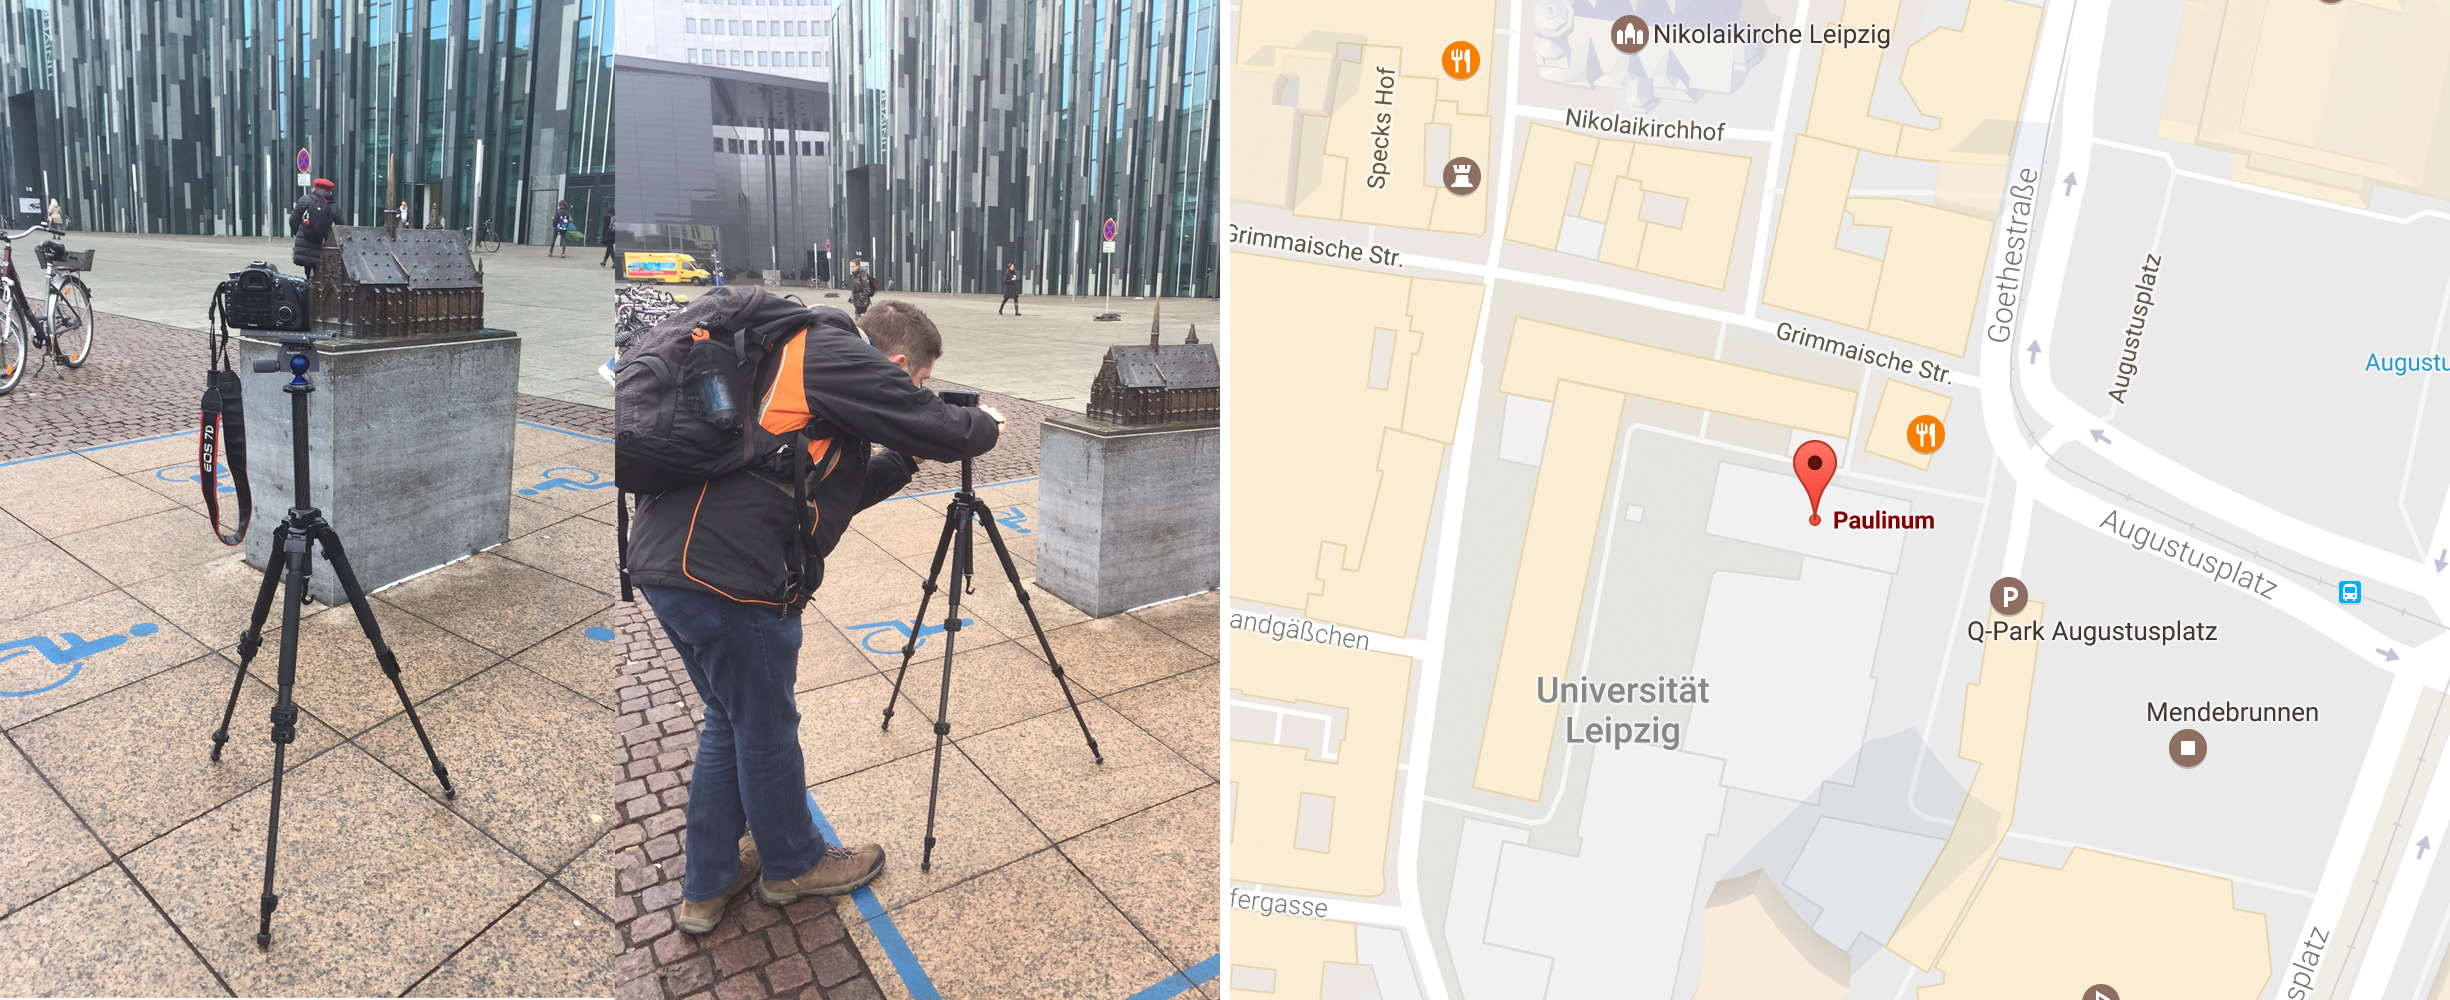
\includegraphics[width=\linewidth]{img/places/paulinum.jpg}
			\caption{Aufnahmesituation und -ort Paulinum}
			\label{img:paulinum_map}
		\end{figure}

		\subsubsection{Kameraeinstellungen}
				\begin{tabular}{ll}
					\textbf{Kamera:} &\textbf{Canon EOS 7D} \\
					Objektiv: &Canon EF 10-22mm F/3.5-4.5 USM\\		
					Brennweite:& 22mm \\
					Belichtungszeit: & $\frac{1}{13}$s /$\frac{1}{13}$s\\
					Blendenwert: & f/8\\
					Empfindlichkeit & ISO 100 \\
				\end{tabular}\\
				
				\begin{tabular}{ll}
					\textbf{Kamera:} &\textbf{Fujifilm Finepix Real 3D} \\
					Brennweite:& 35 mm \\
					Belichtungszeit: & $\frac{1}{70}$s / $\frac{1}{70}$s\\
					Blendenwert: & f/3,7\\
					Empfindlichkeit & ISO 100 \\
				\end{tabular}\\


	\subsubsection{Vorgehen}
	Die Kameras wurden so ausgerichtet, dass sie vertikal mit der Skulptur auf gleicher Höhe liegen. Außerdem wurden sie etwas seitlich positioniert (siehe Abbildung \ref{img:paulinum_map}), sodass der neue Universitätscampus im Hintergrund erkennbar ist. Sie wird dabei von der Fassade des neuen Paulinum eingerahmt, sodass ein geschichtlicher, aber auch ein farblicher Kontrast entsteht. Die Aufnahmen entstanden am 25.01.2017 um 14:37 Uhr. 
	
	\newpage
	\begin{figure}[h]
		
\includegraphics[width=\linewidth]{img/ph.jpg}
		\caption{Stereo-Aufnahme Paulinum (Canon EOS 7D)}
	\end{figure}
	
		\newpage
		\begin{figure}[h]
			
\includegraphics[width=\linewidth]{img/ph.jpg}
			\caption{Stereo-Aufnahme Paulinum (Fujifilm Finepix Real 3D)}
		\end{figure}

\section{Dr. Karl-Heine-Denkmal}
\label{sec:palme}
\subsubsection{Aufnahmeort und -idee}
Das Karl-Heine-Denkmal wurde zu ehren des Industriepioniers und Rechtsanwalts Dr.jur. Ernst Carl Erdmann Heine errichtet wurde. Die spätere schreibweise \textit{Karl} entstand aus einer falsch verstandenen Rechtschreibreform heraus. Das Denkmal befindet sich am südlichen Ende der Käthe-Kollwitz-Straße, direkt am Elsterfluttbett. Es wurde am 20. April 1897, zu ehren des Unternehmers, welcher viele Teile des Leipziger Westens urbar gemacht hatte, eingeweiht. Ursprünglich befand sich die Satue auf der nördlichen Seite der Straße, am Eingang zum Palmengarten, wurde aber 1938 auf die Südseite umgesetzt. 1942 wurde im Zuge der Aufrüstung Deutschlands die Bronzestatue abgenommen und eingeschmolzen. Erst im Jahr 2001 wurde eine Nachbildung des originalen Denkmals auf dem erneuerten Sockel montiert. 

		\begin{figure}[H]
			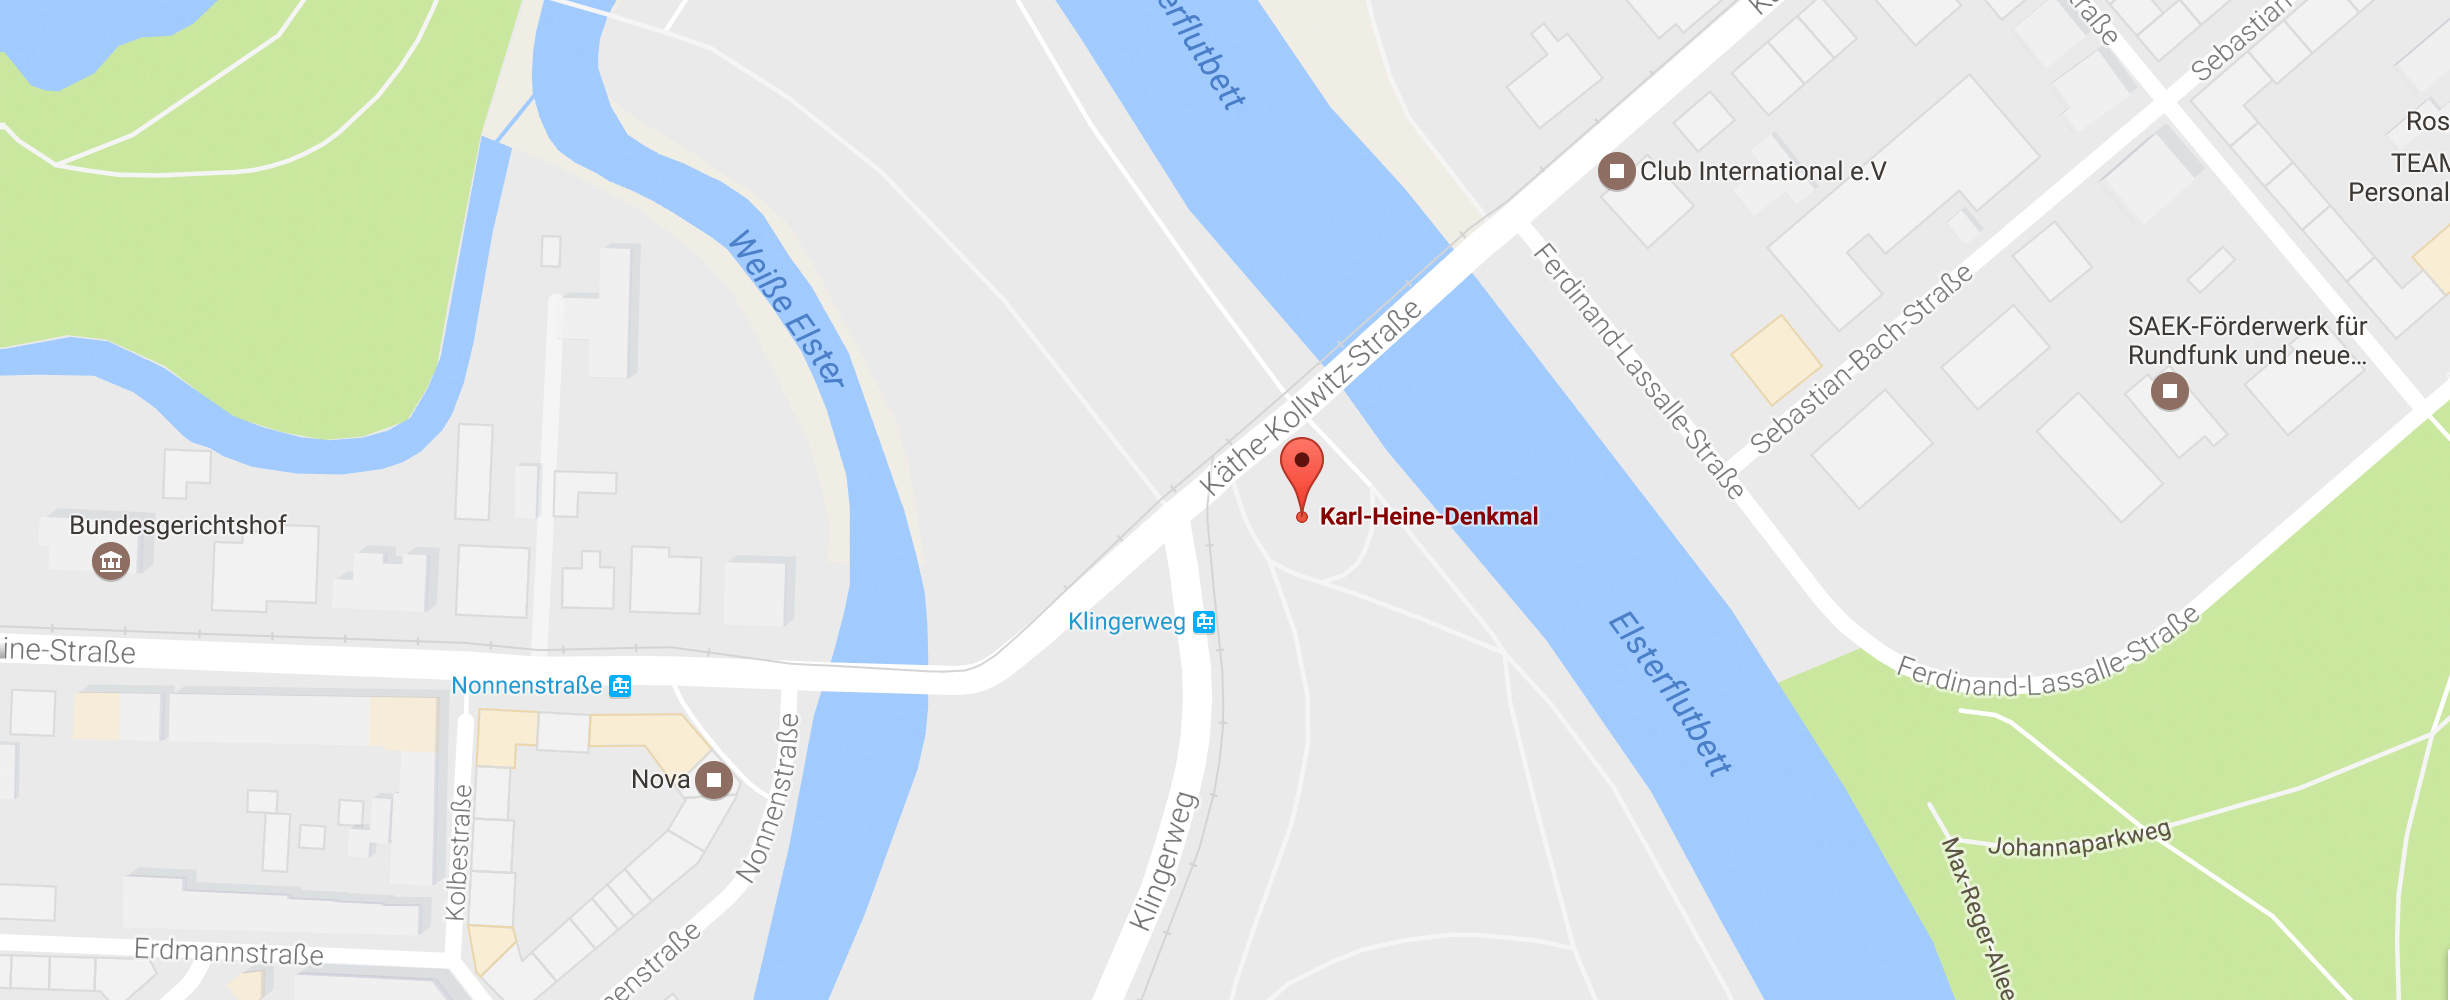
\includegraphics[width=\linewidth]{img/places/kh.jpg}
			\caption{Aufnahmesituation und -ort Dr. Karl-Heine-Denkmal}
			\label{img:kh}
		\end{figure}
		
		\subsubsection{Kameraeinstellungen}
		\begin{tabular}{ll}
			\textbf{Kamera:} &\textbf{Canon EOS 7D} \\
			Objektiv: &Canon EF 10-22mm F/3.5-4.5 USM\\		
			Brennweite:& 22mm \\
			Belichtungszeit: & $\frac{1}{30}$s /$\frac{1}{30}$s\\
			Blendenwert: & f/8\\
			Empfindlichkeit & ISO 100 \\
		\end{tabular}\\
		
		\begin{tabular}{ll}
			\textbf{Kamera:} &\textbf{Fujifilm Finepix Real 3D} \\
			Brennweite:& 35 mm \\
			Belichtungszeit: & $\frac{1}{170}$s / $\frac{1}{170}$s\\
			Blendenwert: & f/3,7\\
			Empfindlichkeit & ISO 100 \\
		\end{tabular}\\


\subsubsection{Vorgehen}
Die Aufnahmen entstanden am 25.01.2017 um 15:17 Uhr. Die Kameras wurden zentral vor dem Denkmal platziert und vertikal nach oben geneigt, um die Statue bei einer Höhe von 3,5m vollständig abzulichten. Aufgrund des einheitlichen grauen Himmels entsteht ein sehr starker Kontrast zwischen Hinter- und Vordergrund, sodass die Statue gut herausgestellt wird.

\newpage
\begin{figure}[h]
	
\includegraphics[width=\linewidth]{img/ph.jpg}
	\caption{Stereo-Aufnahme Karl-Heine-Denkmal (Canon EOS 7D)}
\end{figure}

\newpage
\begin{figure}[h]
	
\includegraphics[width=\linewidth]{img/ph.jpg}
	\caption{Stereo-Aufnahme Karl-Heine-Denkmal (Fujifilm Finepix Real 3D)}
\end{figure}

\section{Leipziger Österreicher-Denkmal}
\label{sec:nikolai}
\subsubsection{Aufnahmeort und -idee}
Die sogenannten Österreicher Denkmäler, sind vier identische Statuen, welche an verschiedenen Stellen in Leipzig zu finden sind. Sie erinnern an die erfolgreiche Teilnahme der Österreicher, bei der Völkerschlacht bei Leipzig. Bis auf die Inschriften, sind die Denkmäler optisch vollkommen gleich. Das für die Stereo-Aufnahme abgelichtete Denkmal befindet sich im Leipziger Südwesten, direkt an der Antonienstraße. Die Inschrift lautet:

\bigskip
\begin{center} 
	\textit{Oesterr. 3. Korps | Feldzeugmeister Graf Gyulai | 1. leichte Division Feldmarschalleutnant | Prinz Moritz Liechtenstein | Detachement Oberstlt. Frh. v. Simbschen\\
		Dem Andenken der in den Kämpfen bei Lindenau, Zschocher u. Schleussig gefallenen Helden.} 
\end{center}

\bigskip
Auf dem qudratischen Sockel erhebt sich ein Doppeladler, also ein Adler mit zwei Köpfen, welcher auf einem Schwert steht und die Kronen der österreichisch-ungarischen Doppelmonarchie trägt. 

		\begin{figure}[H]
			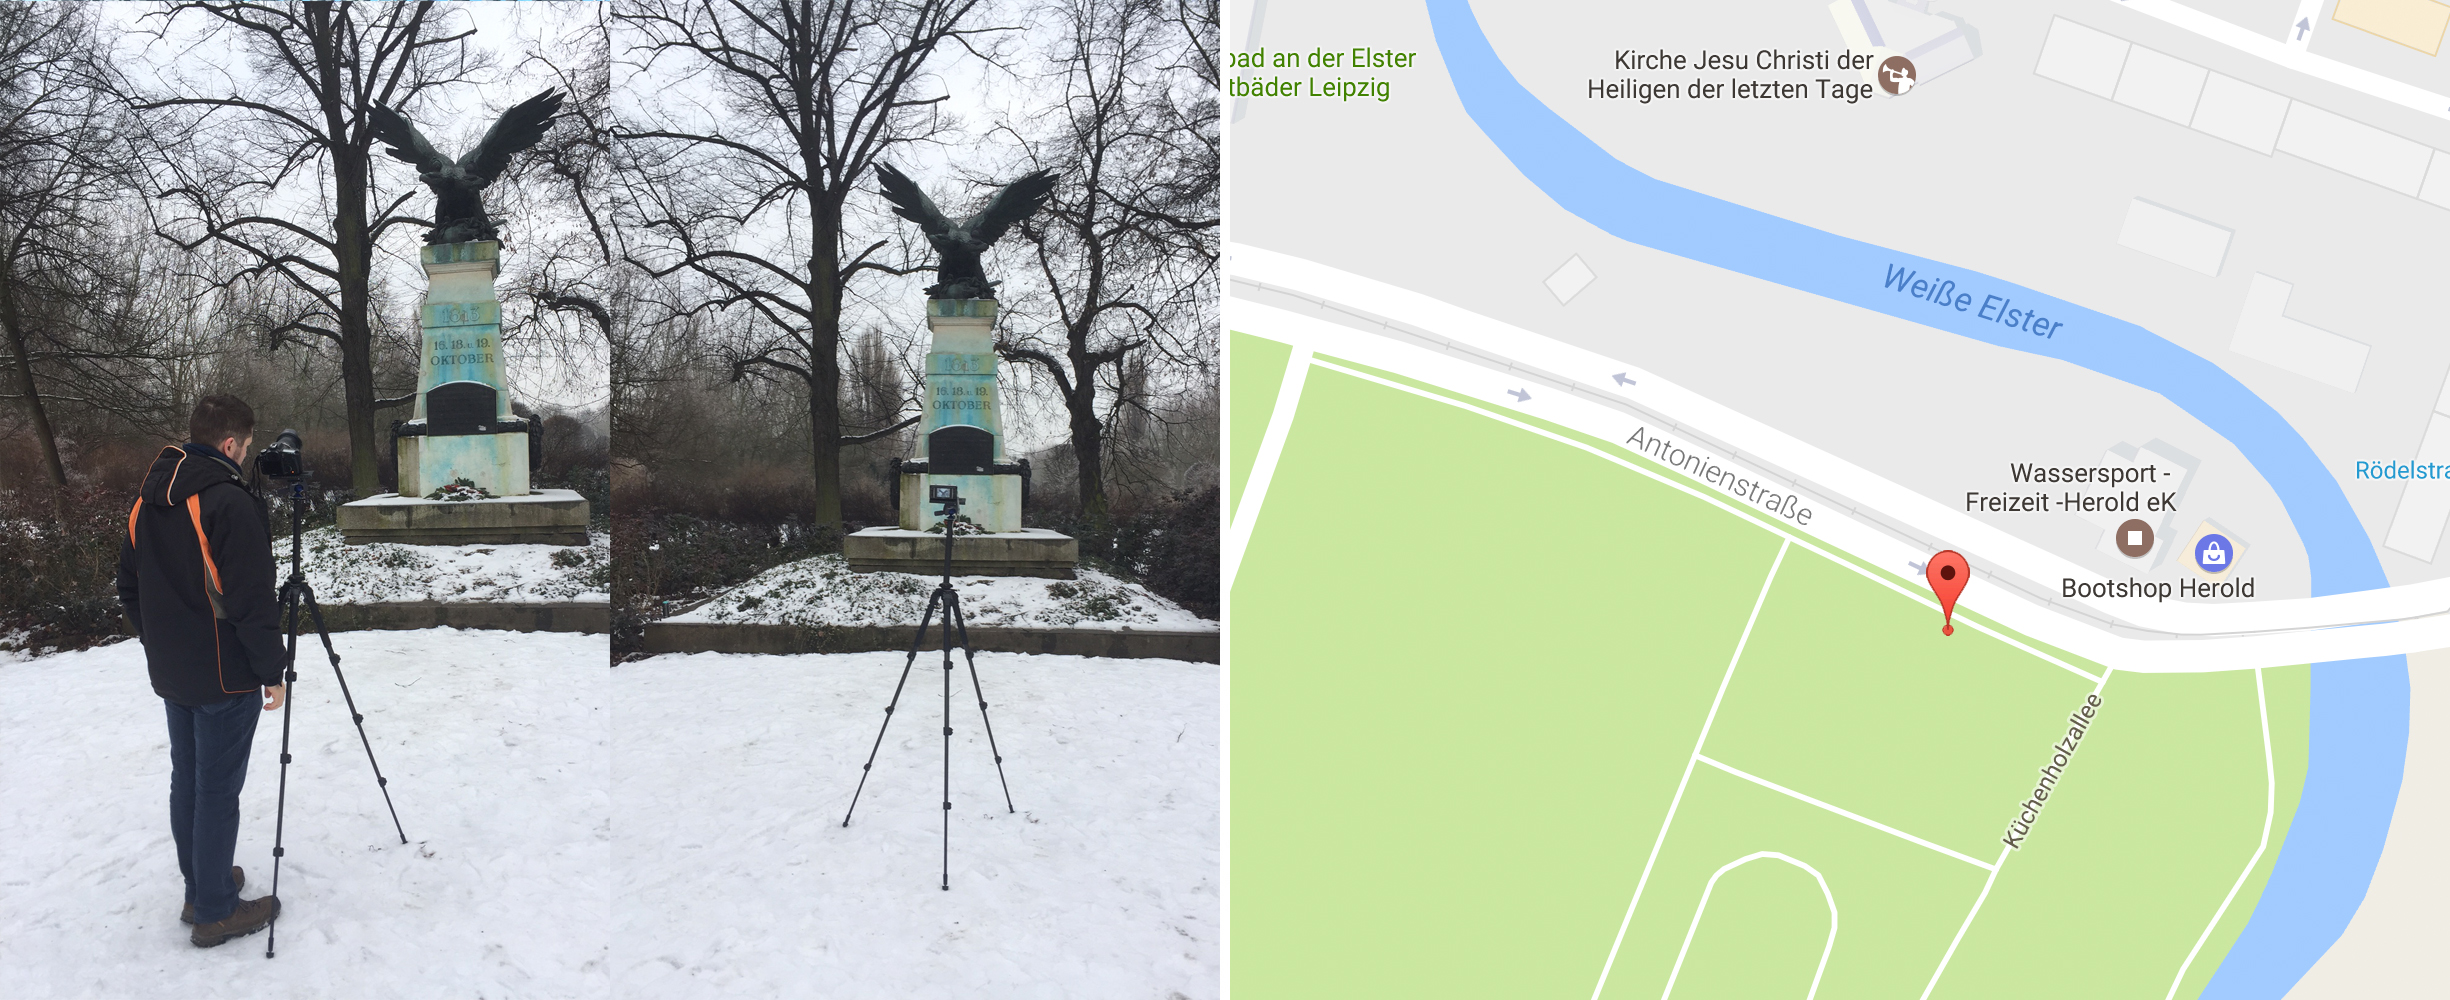
\includegraphics[width=\linewidth]{img/places/oer.jpg}
			\caption{Aufnahmesituation und -ort Österreicher-Denkmal}
			\label{img:oer}
		\end{figure}
		
		\subsubsection{Kameraeinstellungen}
		\begin{tabular}{ll}
			\textbf{Kamera:} &\textbf{Canon EOS 7D} \\
			Objektiv: &Canon EF 10-22mm F/3.5-4.5 USM\\		
			Brennweite:& 56mm \\
			Belichtungszeit: & $\frac{1}{8}$s /$\frac{1}{8}$s\\
			Blendenwert: & f/8\\
			Empfindlichkeit & ISO 100 \\
		\end{tabular}\\
		
		\begin{tabular}{ll}
			\textbf{Kamera:} &\textbf{Fujifilm Finepix Real 3D} \\
			Brennweite:& 35 mm \\
			Belichtungszeit: & $\frac{1}{150}$s / $\frac{1}{150}$s\\
			Blendenwert: & f/4\\
			Empfindlichkeit & ISO 200 \\
		\end{tabular}\\


\subsubsection{Vorgehen}
Ähnlich wie im Abschnitt \ref{sec:palme} bereits beschrieben, wurden auch bei dieser Aufnahme die Kameras so platziert, dass sie zentral auf das Denkmal schauen. Aufgrund der Höhe der Statue, sowie der räumlichen Begrenzung durch die Straße musste ein relativ steiler vertikaler Winkel eingestellt werden. Außerdem sollte nur der Adler und nicht das gesamte Denkmal eingefangen werden, sodass der optische Zoom der Fujifilm Finepix genutzt wurde. Die Aufnahmen entstanden am 25.01.2017 um 15:46 Uhr. Aufgrund der Wetterlage und des grauen Himmels ergibt sich ein starker Hell-Dunkel-Kontrast wodurch sich der Doppeladler in der realisierten Stereoaufnahme besonders gut vom restlichen Hintergrund abhebt. 

\newpage
\begin{figure}[h]
	
\includegraphics[width=\linewidth]{img/ph.jpg}
	\caption{Stereo-Aufnahme Österreicher-Denkmal (Canon EOS 7D)}
\end{figure}

\newpage
\begin{figure}[h]
	
\includegraphics[width=\linewidth]{img/ph.jpg}
	\caption{Stereo-Aufnahme Österreicher-Denkmal (Fujifilm Finepix Real 3D)}
\end{figure}
	
	\section{Goethedenkmal -- Alte Handelsbörse}
	\label{sec:wagner}
	\subsubsection{Aufnahmeort und -idee}
	Wie in vielen deutschen Städten, in denen Goethe gewirkt und gelebt hat, steht auch in Leipzig ein Denkmal von Johann Wolfgang von Goethe. Das Denkmal befindet sich am Leipziger Naschmarkt und zeigt Goethe als jungen Mann. Es erinnert an das dreijährige Studium Goethes in Leipzig und beruht auf einem Entwurf von Carl Seffner. Der Sockel trägt auf der Vorder- beziehungsweise Rückseite die beiden Inschriften:
	
	\bigskip
	\begin{center} 
		\textit{Johann Wolfgang Goethe} 
		
		\textit{Student in Leipzig 1765–68} 
	\end{center}
	
	\bigskip
	Unmittelbar hinter dem Denkmal befindet sich die Alte Handelsbörse, welches eines der ältesten Bauwerke Leipzigs ist. Die Initiative zum Bau dieses Gebäudes ging von Großkaufleuten aus, da man einen neutralen Ort brauchte um Geschäfte zu besiegeln und zum Abschluss zu bringen. 
	
			\begin{figure}[H]
				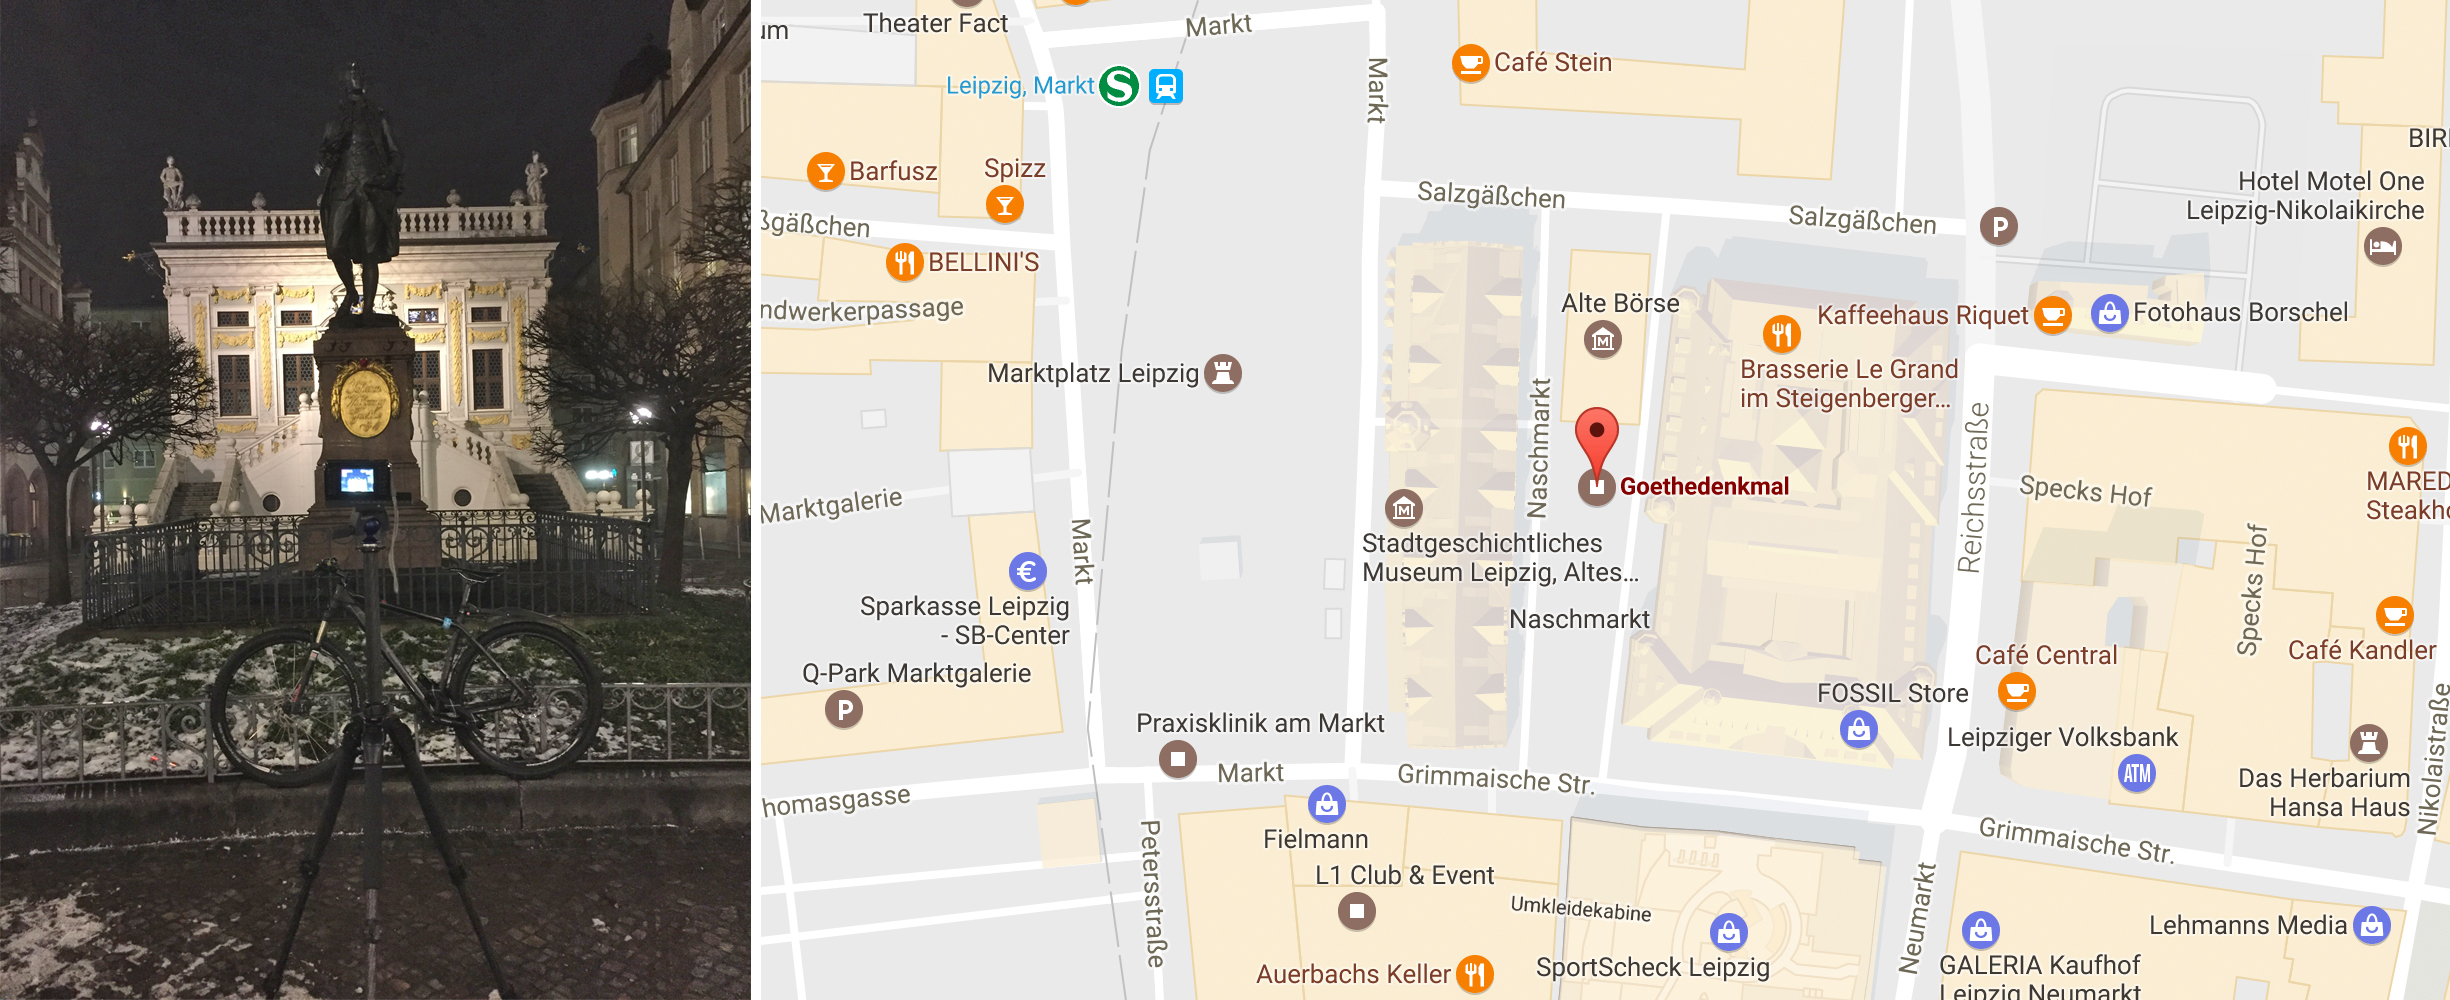
\includegraphics[width=\linewidth]{img/places/goe.jpg}
				\caption{Aufnahmesituation und -ort Goethedenkmal}
				\label{img:oer}
			\end{figure}
			
			\subsubsection{Kameraeinstellungen}
			\begin{tabular}{ll}
				\textbf{Kamera:} &\textbf{Canon EOS 7D} \\
				Objektiv: &Canon EF 10-22mm F/3.5-4.5 USM\\		
				Brennweite:& 22mm \\
				Belichtungszeit: & 8s / 8s\\
				Blendenwert: & f/8\\
				Empfindlichkeit & ISO 100 \\
			\end{tabular}\\
			
			\begin{tabular}{ll}
				\textbf{Kamera:} &\textbf{Fujifilm Finepix Real 3D} \\
				Brennweite:& 35 mm \\
				Belichtungszeit: & $\frac{1}{5}$s / $\frac{1}{5}$s\\
				Blendenwert: & f/3,7\\
				Empfindlichkeit & ISO 400 \\
			\end{tabular}\\
	
	\subsubsection{Vorgehen}
	Die Aufnahmen entstanden am 25.01.2017 um 17:45. Die Kameras wurden erneut zentral vor dem Denkmal platziert. Die Alte Handelsbörse ist im Hintergrund und bildet einen hellen Rahmen um die Statue von Johann Wolfgang von Goethe, sodass sich diese, aufgrund des vorherrschenden Kontrastes, sehr gut abhebt. Die Indirekte Beleuchtung sorgt für eine angenehme, warme Atmosphäre und die historische Alte Handelsbörse erlaubt einen Einblick, wie es zur Zeit Goethes in Leipzig gewesen sein könnte. 

	 \newpage
	 \begin{figure}[h]
		 	
\includegraphics[width=\linewidth]{img/ph.jpg}
		 	\caption{Stereo-Aufnahme Goethedenkmal (Canon EOS 7D)}
	 \end{figure}
	 
	 \newpage
	 \begin{figure}[h]
 	 	
\includegraphics[width=\linewidth]{img/ph.jpg}
 	 	\caption{Stereo-Aufnahme Goethedenkmal (Fujifilm Finepix Real 3D)}
	 \end{figure}

	

	\chapter{Nachbearbeitung und Entwicklung}
		Die Fotos der digitalen Spiegelreflexkamera (DSLR) liegen jeweils in 2 Formaten vor. Als JPG und RAW. Aufgrund dessen werden die Raw-Dateien vor der eigentlichen Zusammenstellung in ein Fotobearbeitungsprogramm, wie z. B. Lightroom, geladen. Dort erfolgt die Optimierung beider Bilder, wobei darauf geachtet wird, dass beide auf dieselbe Weise anzupassen sind. Zu den Bearbeitungsschritten zählt ua. das Anheben der Schatten, um z. B. die Goethe-Statue vor der Börse herauszuarbeiten. Anschließend erfolgt das Speichern der bearbeiteten Bilder als JPG und der Import dieser in das Programm \textit{StereoPhoto Maker}.
		\newpage
		Die Abbildung \ref{img:maker_import} veranschaulicht die Import-Möglichkeiten dieser Software. Für das Öffnen der MPO-Dateien, kann man direkt auf \grqq{}Stereobild öffnen...\grqq{} klicken. Die mit der DSLR aufgenommenen Fotos hingegen werden über \grqq{}Linkes/Rechtes Bild öffnen...\grqq{} importiert.
		\begin{figure}[H]
			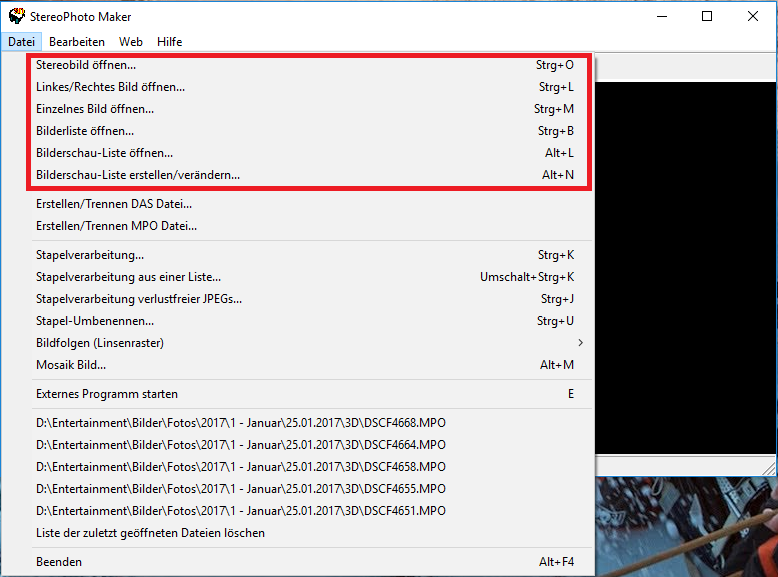
\includegraphics[width=\linewidth]{img/steps/step1.png}
			\caption{StereoPhoto Maker - Import}
			\label{img:maker_import}
		\end{figure}
	
		Nach dem Import der Bilder, werden beide Fotos Seite an Seite angezeigt. Auf der Benutzeroberfläche kommen zusätzliche Bearbeitungsbuttons hinzu. Die wichtigsten zeigt die Abbildung \ref{img:maker_options}. So ist es möglich über den blau markierten Button eine erste 3D-Vorschau zu erzeugen. Dort sind viele Optionen für die 3D-Darstellung vorhanden, wie z. B. die Technik für Shutterbrillen oder auch ältere, wie die Grau- und Farb-Anaglyphentechnik. Sollten beide Fotos vertauscht sein, ist eine Korrektur über den grün gekennzeichneten Knopf möglich.
				
		\begin{figure}[H]
			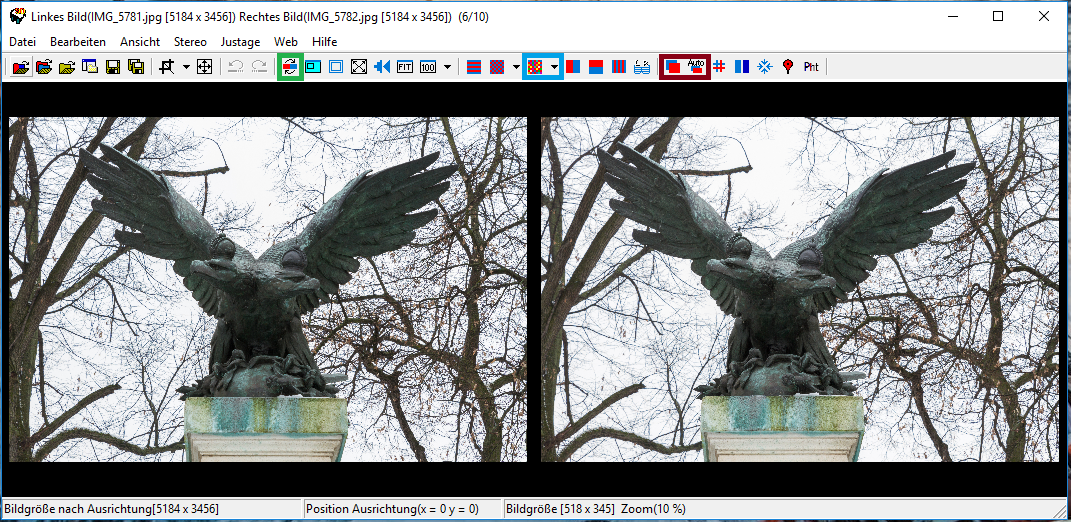
\includegraphics[width=\linewidth]{img/steps/step2.png}
			\caption{StereoPhoto Maker - Darstellung und Optionen}
			\label{img:maker_options}
		\end{figure}

		Zuletzt erfolgt eine Feinjustage der Einzelbilder. Dies kann automatisch geschehen oder auch manuell gesteuert werden. Die rote Markierung zeigt die Position beider Möglichkeiten in der GUI. Bei der Justage werden beide Bilder im richtigen Winkel zueinander gedreht und die Abstände der Fotos angepasst. Dabei geht hervor, dass die Autojustage extrem gut funktioniert, wenn beide Fotos mit einem Stativ geschossen wurden. Dies zeigt der Justage-Dialog (Abb. \ref{img:maker_justage}) hervor, anhand dessen die Bilder nur sehr geringfügig justiert werden müssen.
		
		\begin{figure}[H]
			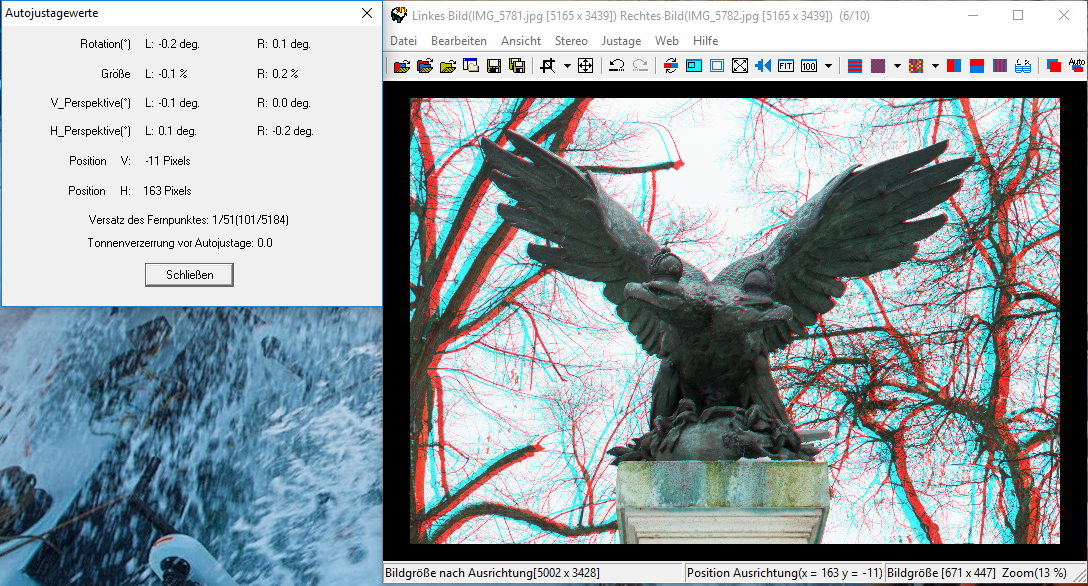
\includegraphics[width=\linewidth]{img/steps/step3.png}
			\caption{StereoPhoto Maker - Autojustage und Zusammenführung}
			\label{img:maker_justage}
		\end{figure}
		
		Sollte die Autojustage kein zufriedenstellendes Ergebnis liefern, hat der Nutzer die Möglichkeit, dies manuell zu tun. Wie in der Abbildung \ref{img:maker_manual} zu sehen ist, kann auf die vertikale und horizontale Verschiebung über die orange bzw. rot markierten Slider Einfluss genommen werden. In der grünen Box besteht die Möglichkeit den Drehwinkel anzupassen. Alle Änderungen erwirken ein Updaten der Vorschau und somit das Darstellen der aktuellen Einstellungen.
		
		\begin{figure}[H]
			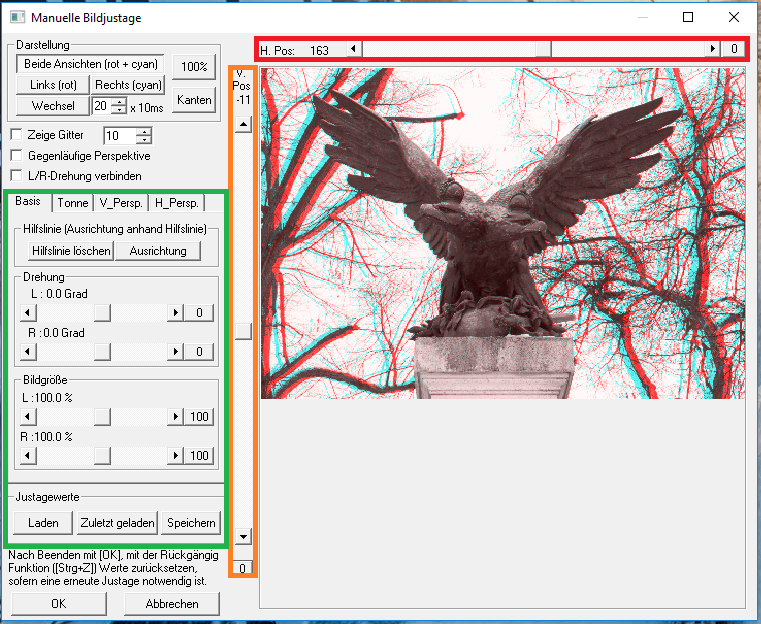
\includegraphics[width=\linewidth]{img/steps/step4.png}
			\caption{StereoPhoto Maker - Manuelle Bildjustage}
			\label{img:maker_manual}
		\end{figure}
	
		Nach der Justage kann das Foto in gängigen Fotoformaten exportiert werden. Da zum Betrachten eine rot-cyan Brille zum Einsatz kommt, wendet man die rot-cyan Grau-Anaglyphentechnik auf die Fotos an.

	\chapter{Fazit}
		Zusammenfassend lässt sich sagen, dass die kleine Kompaktkamera bei guten Lichtbedingungen anschauliche Fotos erzeugen kann. Zudem liegen diese Bilder direkt in einem kompatiblen 3D-Format vor und somit ist ein schnelles, problemloses Einlesen in die entsprechenden Programme möglich. Die Kehrseiten der Kamera sind die sehr umständliche Menüführung mit verschachtelten Unterkategorien. Außerdem stößt man mit dieser Kamera sehr schnell an die Grenzen der Hardware, wobei Langzeitbelichtungen nicht möglich sind und der Sensor nicht besonders hoch aufgelöst (10MP) ist.
		Bei der Verwendung einer DSLR, hier Canon 7D, kann man alle Vorteile eines solchen Systems genießen. Der Sensor ist hochauflösender, die Objektive wechselbar, zudem sind alle manuellen Einstellungsmöglichkeiten wählbar. Aufgenommene Fotos können in RAW aufgenommen und vor dem Zusammenfügen nahezu verlustfrei nachbearbeitet werden. Auch der Import der Bilder in das 3D-Erzeugungsprogramm stellt kein Problem dar. Der einzige richtige Nachteil gegenüber der Kompaktkamera ist, dass ein Stativ mit entsprechendem Kopf notwendig ist, um die Fotos im richtigen Abstand voneinander zu erzeugen. Schnappschüsse können somit nicht erstellt werden. Auch bewegte Objekte sind mit der DSLR, aufgrund der Versatzzeit, ein Problem. Die Kompakte hingegen schießt zwei Fotos simultan und ist somit für ein solches Szenario geeignet.
		
	
\end{document}